 
\renewcommand\chapname{Grammars via PAWS and XLingPaper}	
\renewcommand\longchapname{Grammars for the people, by the people, made easier using  PAWS  and  XLingPaper}
\renewcommand\shortauthor{Cheryl A. Black and H. Andrew Black}
\renewcommand\longauthor{Cheryl A. Black and H. Andrew Black \\SIL International and University of North Dakota}
\chapter*{\longchapname}
\chapterauthor{\longauthor}
\mytoc{}
 

\begin{abstract}


The task of documenting the minority languages of the world, many of them endangered, is daunting. Further, it is most likely impossible to expect that linguists can go to every language and write a reference grammar for it. At the same time, the indigenous people are becoming more educated and more interested in working on their own languages. This paper describes a computational tool that teaches native speakers about various linguistic constructions, has them enter data from their language and answer simple questions about it, and then produces a draft of a practical grammar of the language. This grammar can be edited for publishing electronically and/or on paper and is useful for the people themselves as well as by linguists.

The underlying XML technology  allows much of the complexity to be hidden from the user, while providing multiple views and outputs possible from the same data. The marked-up XML files are archivable and usable by many XML editors. Localization and customization are also possible. 

\end{abstract}

\section{Introduction}\label{sIntro}
Linguists are scrambling to try to meet the need of documenting and describing the endangered languages of the world, as well as many of the other minority languages. Further, it is fair to assume it would be impossible for linguists to go to every language and write a reference grammar for it. The task simply takes too much time and there are not enough trained linguists available. Even if the linguists could accomplish the task of language documentation and description, current methods would not be productive enough, since documents written in English for linguists do little to help preserve a language.

At the same time, the indigenous people want to be involved as they are becoming more educated and more interested in working on their own languages. A different type of grammar is needed: one that serves the language community, describes the language in general terms, and is also useful to linguists for extracting data for analysis. This type of grammar has the potential to revitalize the use of a language as the people realize their language is a ``real'' language worthy of use because it has a grammar and a dictionary like the national language.

This paper describes a computational tool called {PAWS} (Parser and Writer for Syntax) that can be used, especially in a workshop setting, to teach native speakers about various linguistic constructions, have them enter data from their language and answer simple questions about it, and then produce a draft of a practical grammar of the language. Currently {PAWS} only runs on Windows operating systems. It is available at \url{http://carla.sil.org/paws.htm}.

The practical grammar style is illustrated in section \ref{sPractical}. Section \ref{sInterface} details the user interface for input and how to edit the output using the XLingPaper authoring tool \citep{rXLingPaper}.\footnote{\label{nXLingPaper}
   For more on XLingPaper, see \url{http://www.xlingpaper.org/}.
} 
Section \ref{sComp} then explains how it all works computationally.

\section{Practical grammars}\label{sPractical}
Practical grammars, also known as popular grammars, are designed for use by the native speakers in the language community. As such, the grammars should be written using the national language for the explanations and glosses. The version described here includes additional material to provide some pedagogy for the reader. Moreover, numerous tables and data in interlinear format and description of the constructions make it useful to linguists and bilingual teachers as well.


\subsection{General structure}\label{sPracticalStructure}
A practical grammar consists mostly of data with some prose explanation. Information about single words or morphemes is usually presented in tables, but all longer examples are given in interlinear format. This format is a bit different than that found in most linguistic publications in order to make it most useful to and understandable by native speakers of the language. Four lines are used: the first line gives the vernacular words, without breaking them into morphemes, as morpheme breaks could be very confusing to the native speaker. The second line is the gloss of the word, with any additional words needed in the gloss language separated by periods. The third line gives the morpheme gloss with normal linguistic abbreviations and conventional symbols like hyphens separating the glosses for each morpheme. This third line is especially for linguists, but is given lower than the word gloss to make it easier for the speakers of the language and bilinguals to skip over if they so choose. The individual morphemes will usually be listed in separate tables to enable the linguists to parse the words, as exemplified in \xref{xIZPossPnDep}-\xref{xIZInflectionFeatures}. (It would also be possible for the author to add a line to the grammar output giving the vernacular morphemes between hyphens, but this should come after the word gloss line and before the morpheme gloss line if included.) Finally, a free translation is given on the fourth line of the interlinear. This four-line structure is illustrated schematically in \xref{xInterlinearEx}.


\let\eachwordtwo=\it
\let\eachwordthree=\rm

\ea  \label{xInterlinearEx}%1
\glll {\sc vernacular words} word word word\\
      {\sc literal word glosses} `gloss' `gloss' `gloss'\\
 {\sc morpheme glosses} `\textsc{pre}-root-\textsc{suf}' `\textsc{pre}-root-\textsc{suf}' `\textsc{pre}-root-\textsc{suf}'\\
 {\sc free translation}  free translation phrase or sentence\\
\z


A completed interlinear example from Isthmus Zapotec is shown in \xref{xInterlinearIZ}:

\ea  \label{xInterlinearIZ}%2
\glll Gudixe Juan chii bexu ri{\saltillo}   lu   bí{\saltillo}chibe\\
paid   John ten  peso those face his.brother\\
\textsc{compl}-pay John ten peso this to brother-\textsc{3pl}\\
 `John paid those ten pesos to his brother.'
\z

One or more tables listing the dependent pronoun forms, as illustrated in Table \ref{xIZPossPnDep} for Isthmus Zapotec, document this information in a central place and aid the linguist in parsing the words in the interlinear examples.\footnote{\label{nIZdata}
 First and second person singular forms are not listed in the table because they cause a change in the noun root. Such details need to be explained separately while editing the grammar output.
}

\glossSTDmode

\begin{table}
\begin{tabular}{lll}
{\textbf{Person}} & {\textbf{Possessor Pronouns}} & {\textbf{Gloss}}\\
{\multirow{2}{*}[1.25ex]{first}} & du & {`ours (exclusive)'}\\
 & nu & {`ours (inclusive)'}\\
{second} & tu & {`yours ({\textsc{pl})'}}\\
{\multirow{6}{*}[6.25ex]{third}} & be & {`his/hers (person)'}\\
 & me & {`his/hers (animal)'}\\
 & ni & {`its (thing)'}\\
 & cabe & {`theirs (persons)'}\\
 & came & {`theirs (animals)'}\\
 & cani & {`its (things)'}\\
\end{tabular}
\caption{Dependent pronoun forms of Isthmus Zapotec}
\label{xIZPossPnDep}%3 
\end{table}

The PAWS interface also asks the user to check off the inflection features used in their language. This is output in a table such as shown in Table \ref{xIZInflectionFeatures} for Isthmus Zapotec.

\begin{table}
\begin{tabular}{lll}
{\textbf{Type of feature}} 	& {\textbf{Feature}} & {\textbf{Form}}\\
{\multirow{7}{*}[7.5ex]{aspect}} & {completive} & {bi-/gu-}\\
				& {habitual} & {r-/ri-/ru-}\\
				& {incompletive (future)} & {za-/zi-/zi-/zu-}\\
				& {perfect} & {hua-/huay-}\\
				& {potential} & {gu-/gui-/Ø}\\
				& {progressive} & {ca-/cay-/cu-}\\
				& {stative} & {na-}\\
{\multirow{2}{*}[1.25ex]{mood}} & {imperative} & {la- }\\
				& {irrealis} & {ni-/ñ-}\\
\end{tabular}
\caption{Isthmus Zapotec inflection features}
 \label{xIZInflectionFeatures}%4
\end{table}

Note that judgments on the grammaticality of data, usually noted by * and ?, are not used in the practical grammar in order to avoid confusion for the language community. Instead, the prose description of the construction is used to make the distribution clear. The prose is meant to be a-theoretical, but complete enough to allow linguists to apply their theory to the data. A descriptive style grammar also has a longer and wider useful life since it is not limited to the applicability of any particular linguistic theory.

At the end of the grammar, we suggest the addition of several native texts from various genres. This not only allows the language community to identify with the grammar, but also provides examples of sentences in a larger discourse context for the linguist. We suggest a three part presentation of each text to best meet the needs of each audience: 
 
\begin{enumerate}
\item Present the text in the vernacular language as a whole first, so the native speakers can appreciate it. 

\item Present the interlinear form, as in the examples throughout the grammar. 

\item Give a free translation as a whole, so the non-native speaker can appreciate more about the culture. 
\end{enumerate}

The output from {PAWS} does not include any such texts, but it does have a section where the user is encouraged to add them.

\subsection{Impact on a language community}\label{sPracticalExperience}
We have mentioned the importance of completing language description for the endangered languages. Even when a language has been described in English and it is not in imminent danger, a practical grammar written for the language community can have a profound impact. This was clearly demonstrated when the first edition of the practical grammar for Isthmus Zapotec was dedicated in January, 1999 \citep{rPickettBlackMarcial1st}.

While Zapotec speakers in general do feel inferior to Spanish speakers, Isthmus Zapotec is the prestige variety of Zapotec. Further, the grammar of the language had been described quite well by Velma Pickett in her dissertation \citep{rPickettDiss} and in a number of other articles. Still, Zapotec speaker Vicente Marcial Cerqueda came to Velma and to Cheryl Black and asked for help in writing a grammar in Spanish for his people. He wanted his people to realize that they did not have to abandon their language and only teach their children Spanish. The grammar needed to be presented in a simple, clear and correct form, so that they could understand that while their mother tongue is distinct from Spanish in many ways, it has a rich and complete structure just like all the other languages of the world.

We are happy to say that Vicente's goals were substantially realized. When the practical grammar was dedicated, there was a big celebration in Juchitán, Oaxaca, Mexico. Over 100 Zapotecs in full native dress crowded into the auditorium of the Casa de la Cultura. The top mariachi band came out of retirement to play for the dedication. The whole program was videotaped and televised later in its entirety throughout the region. The people stood in a long line afterward to purchase their copy of the grammar and have it autographed by all three coauthors. The next day, there was a radio talk show about the grammar. There were speakers from four different varieties of Zapotec on the air. They would open to a particular page and discuss the construction described there, saying for example, ``It says on page 20 that Isthmus has a plural marker {\textit{ca}} before the noun. In my language we say...'' At the church service we attended on Sunday, people were happy that the grammar was presented because they could now use their Zapotec New Testaments in the public church service instead of just reading it at home. Interest and pride in their language was clearly restored.

A further encouragement came the following week when a dedication service was held at the \em Universidad Nacional Autónoma de México \em in Mexico City: One of the speakers from the university commented that this grammar, even though meant for the people, is useful for the Mexican linguists as well because the data is presented in interlinear format and the IPA charts are included. Our goal of producing a single grammar that could meet both needs was accomplished.


\section{What the user sees}\label{sInterface}
Turning now to the implementation of {PAWS}, when the practical grammar option is selected, only the teaching and questions relevant to writing the grammar are presented to the user. There is a series of fifty-seven interactive web pages for the user to complete. The output is a draft of a practical grammar for their language based on their answers and sample data, which is intended to be further edited and enhanced for publishing.


\subsection{Interactive pages}\label{sPages}
The {PAWS} program contains a series of interactive pages which teach some linguistics and then ask questions about the various constructions. The program initially assumes default answers based on the word order typology of the language, but it allows for exceptions.

On most pages, there is a brief instruction on the construction with illustrative examples, then a series of multiple-choice questions about that construction for the language the user is working on. The number of questions asked depends upon how previous questions were answered. These answers are recorded and later used to give the prose explanation about the distribution of the construction in their language. It also asks the user to enter sample data for the various constructions, and records this data for the examples in the grammar.

Figures \ref{xPossesors1}-\ref{xPossessors3} show one such page for how possessors are handled within nominal phrases. We show what the user sees when they have chosen to only produce a practical grammar output. (The {PAWS} program can also produce a PC-PATR grammar output.\footnote{\label{nPC-PATR}
 PC-PATR is an implementation of the unification-based PATR-II computational linguistic formalism \citep{rShieber1986}. In addition, it is augmented with logical constraints on feature nodes and a priority union operation. The "PC" part of the name reflects the fact that it is designed to be used on personal computers (as opposed to mainframe or other large computers common at the time it was written). It is available for MS-DOS, Microsoft Windows, Macintosh, and Unix.
}  See \citet{rMcConnel} for more on PC-PATR.)
   
\clearpage
% \ea  \label{xPossesors1}%5
% 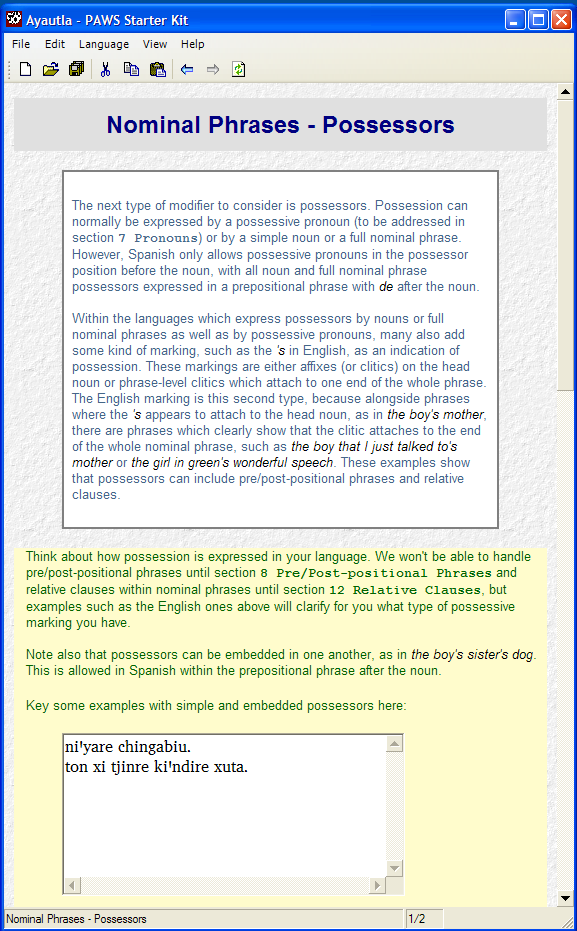
\includegraphics[width=\textwidth]{\imgpath/Possessors.png}
% \z
\begin{figure}[b]
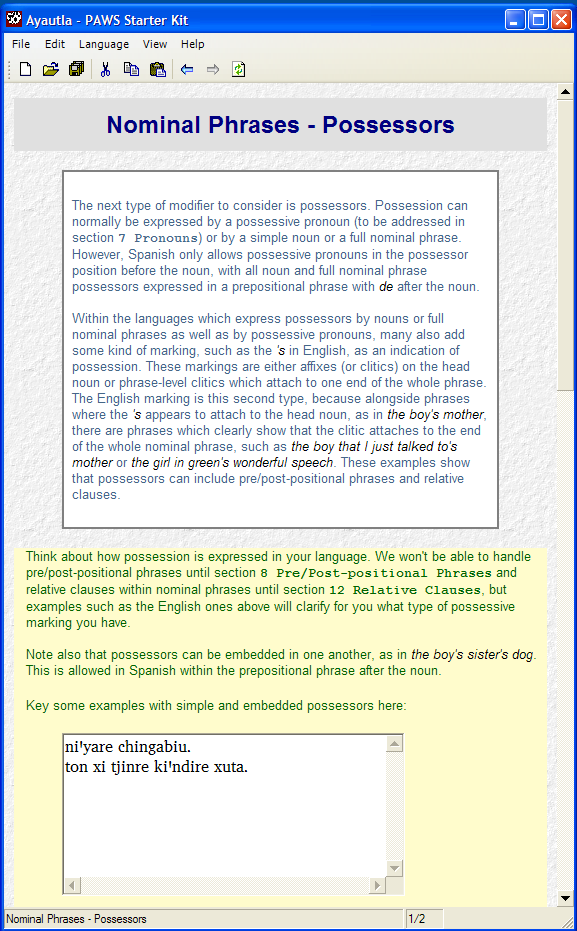
\includegraphics[height=.8\textheight]{\imgpath/Possessors.png} 
\caption{An instruction section along with a request to enter sample data}
\label{xPossesors1}%5
\end{figure}
  
\clearpage
% \newpage
% \ea  \label{xPossessor2}%6
% 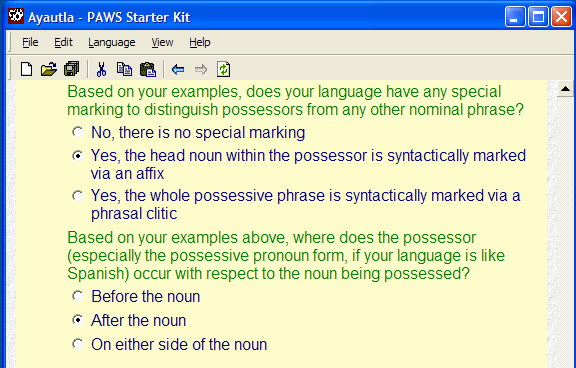
\includegraphics[width=\textwidth]{\imgpath/Possessors2a.png}
% \z
\begin{figure}[t]
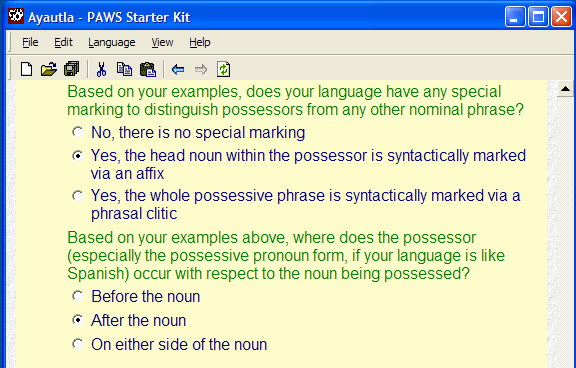
\includegraphics[width=\textwidth]{\imgpath/Possessors2a.png}
\caption{Two sets of multiple choice questions, followed by more instruction and a third multiple choice question.}
 \label{xPossessor2}%6
\end{figure}


\clearpage
% \ea  \label{xPossessor2c}%7
% 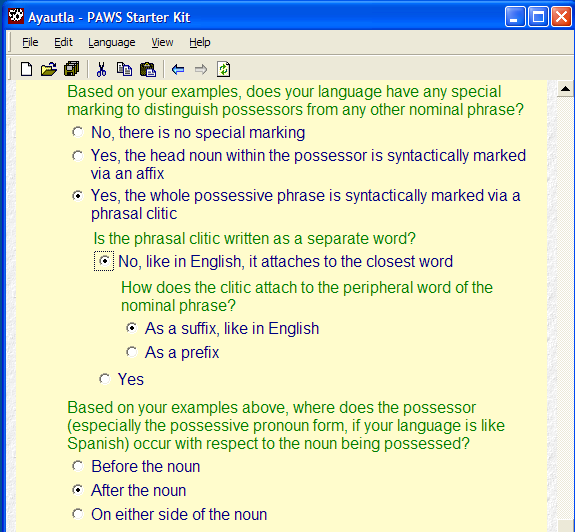
\includegraphics[width=\textwidth]{\imgpath/Possessors2c.png}
% \z
\begin{figure}[t]
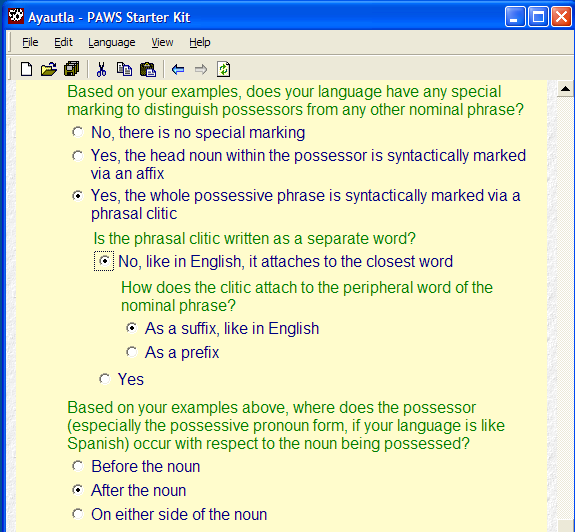
\includegraphics[width=\textwidth]{\imgpath/Possessors2c.png}
\caption{If a user clicks on the second "Yes" answer shown in Figure \ref{xPossessor2}, then more questions are asked (due to the fact that more information is needed about the nature of the phrasal clitic).}
 \label{xPossessor2c}%7
\end{figure}


\clearpage
% \ea  \label{xPossessors2b}%8
% 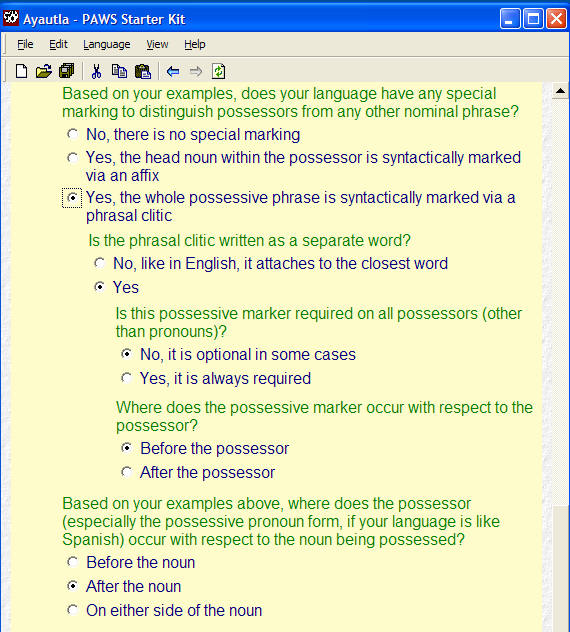
\includegraphics[width=\textwidth]{\imgpath/Possessors2b.png}
% \z
\begin{figure}[p]
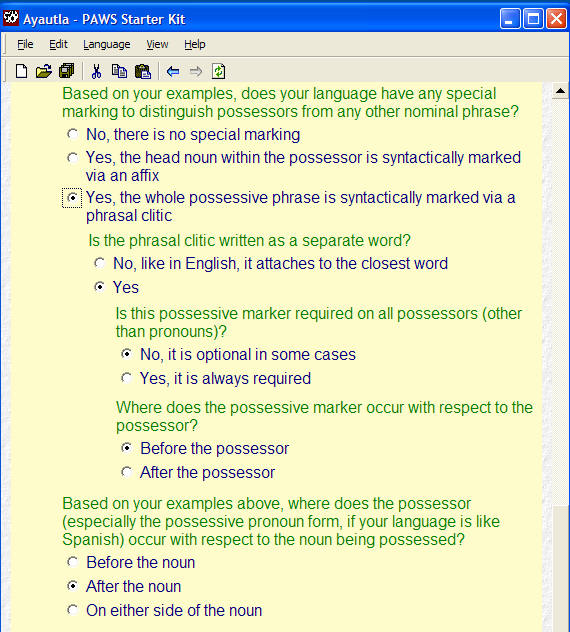
\includegraphics[width=\textwidth]{\imgpath/Possessors2b.png}
\label{xPossessors2b}%8
 \caption{If the user instead chooses the option to say that the phrasal clitic is written as a separate word, then even more questions appear.}
\end{figure} 

\clearpage
% \ea  \label{xPossessors3}%9
% 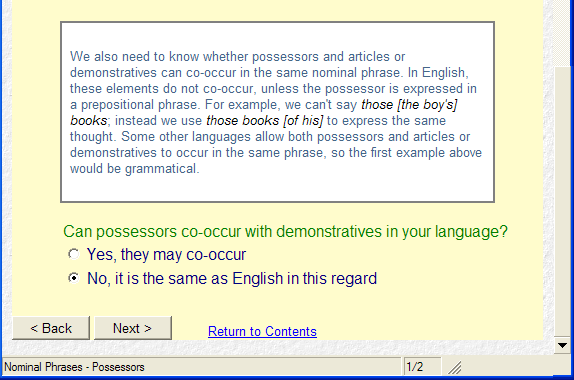
\includegraphics[width=\textwidth]{\imgpath/Possessors3aa.png}
% \z
\begin{figure}[p]
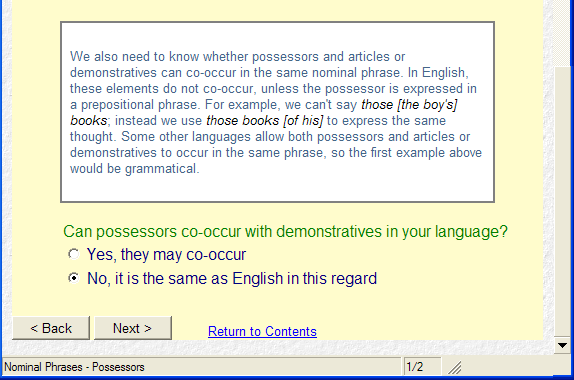
\includegraphics[width=\textwidth]{\imgpath/Possessors3aa.png}
\caption{The bottom portion of the page. It has some instruction, a question, and then two buttons, one for going back to the previous page and the other for going forward to the next page. It also has a link to jump to the main contents page.}
 \label{xPossessors3}%9
\end{figure} 
 \clearpage

\subsection{Grammar draft to edit}\label{sGrammar}
As the user works his/her way through these interactive pages, s/he can save their work and return later for another session. Whenever the work is saved, the output is produced based on the answers given so far. Naturally, we recommend that the user not look at the generated output until s/he has completed all the interactive pages.

Depending on the complexity of the language and how much data is entered, the draft of the practical grammar which is output could be about 60-90 pages if printed out. This includes the prose description and tables and interlinear data.

To illustrate the coverage of the practical grammar, the table of contents for the initial output of one grammar is shown in Figure \ref{xContents} \footnote{\label{nThirdLevelSections}
   In addition to the first and second level sections shown in \xref{xContents}, there are twenty four third level sections.
}

\begin{sidewaysfigure}
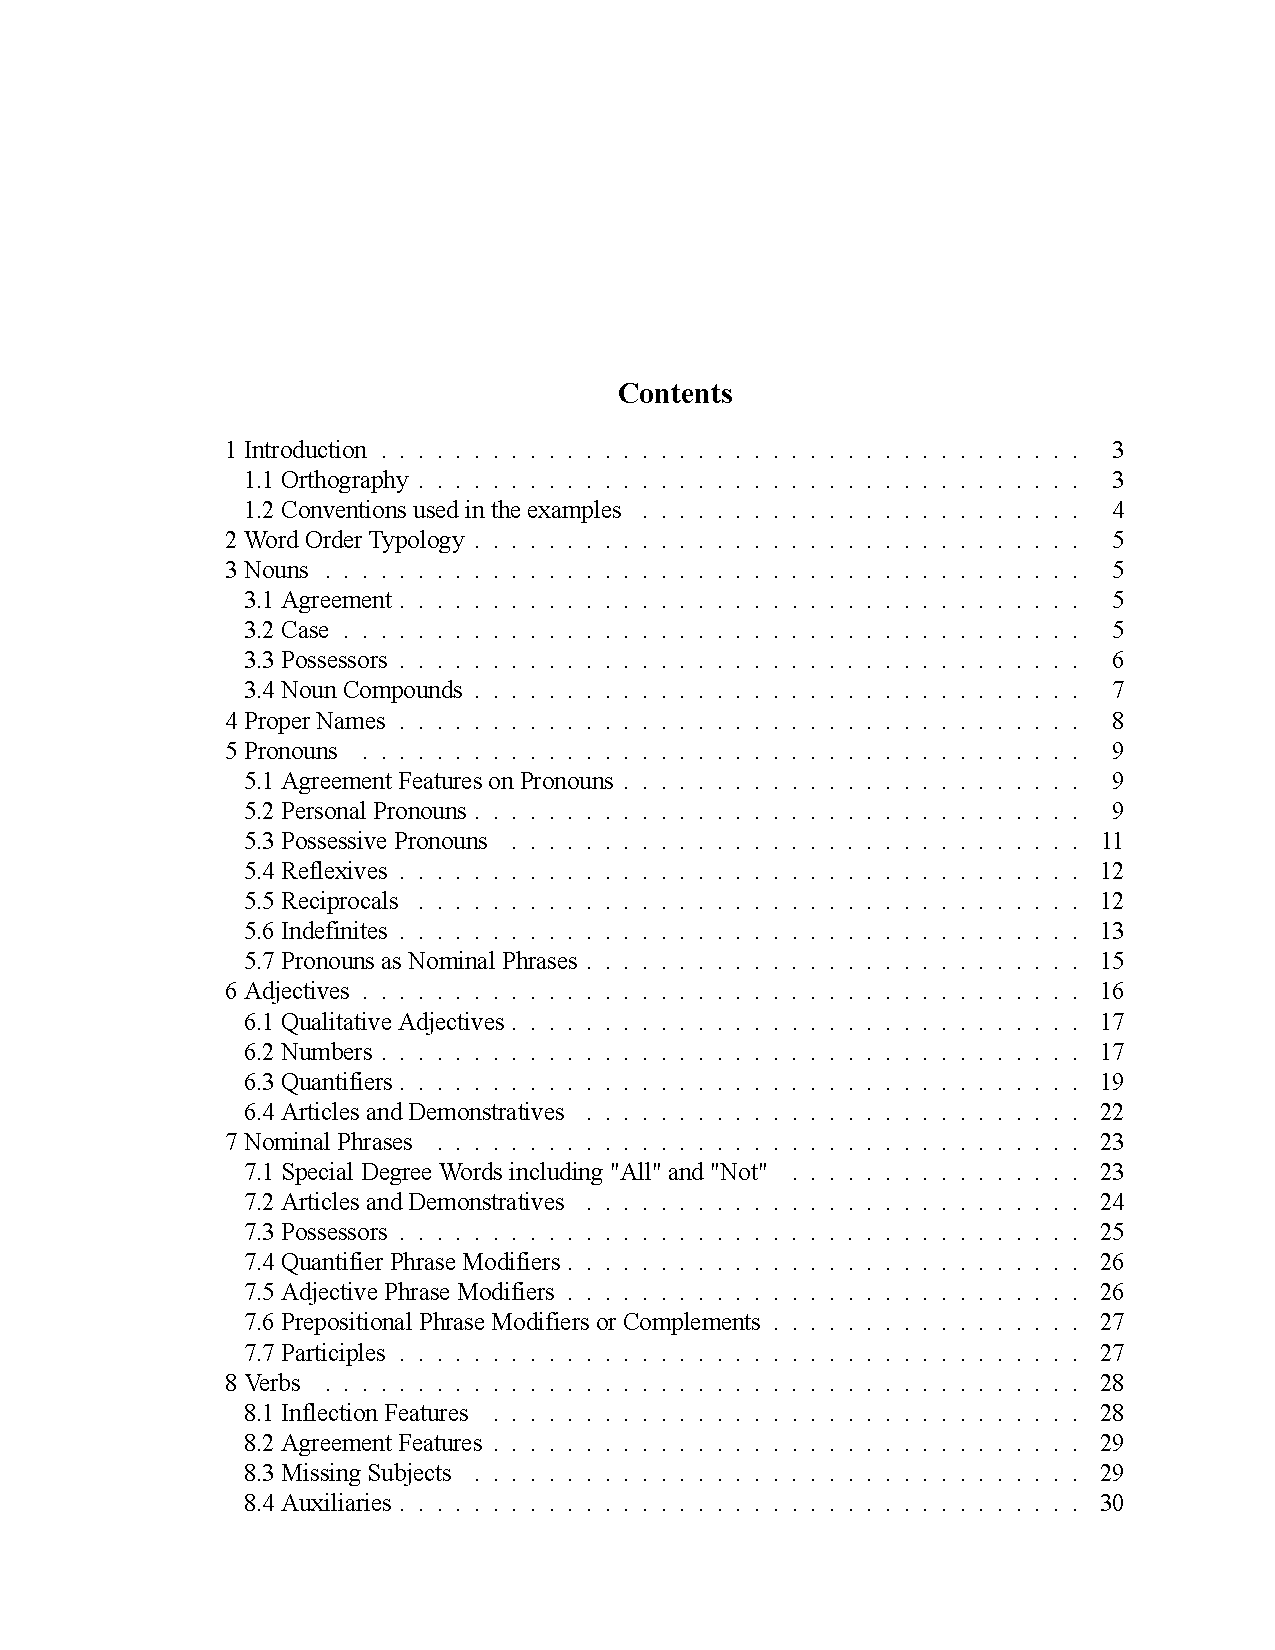
\includegraphics[width=.45\textwidth]{\imgpath/Contents1a.pdf}
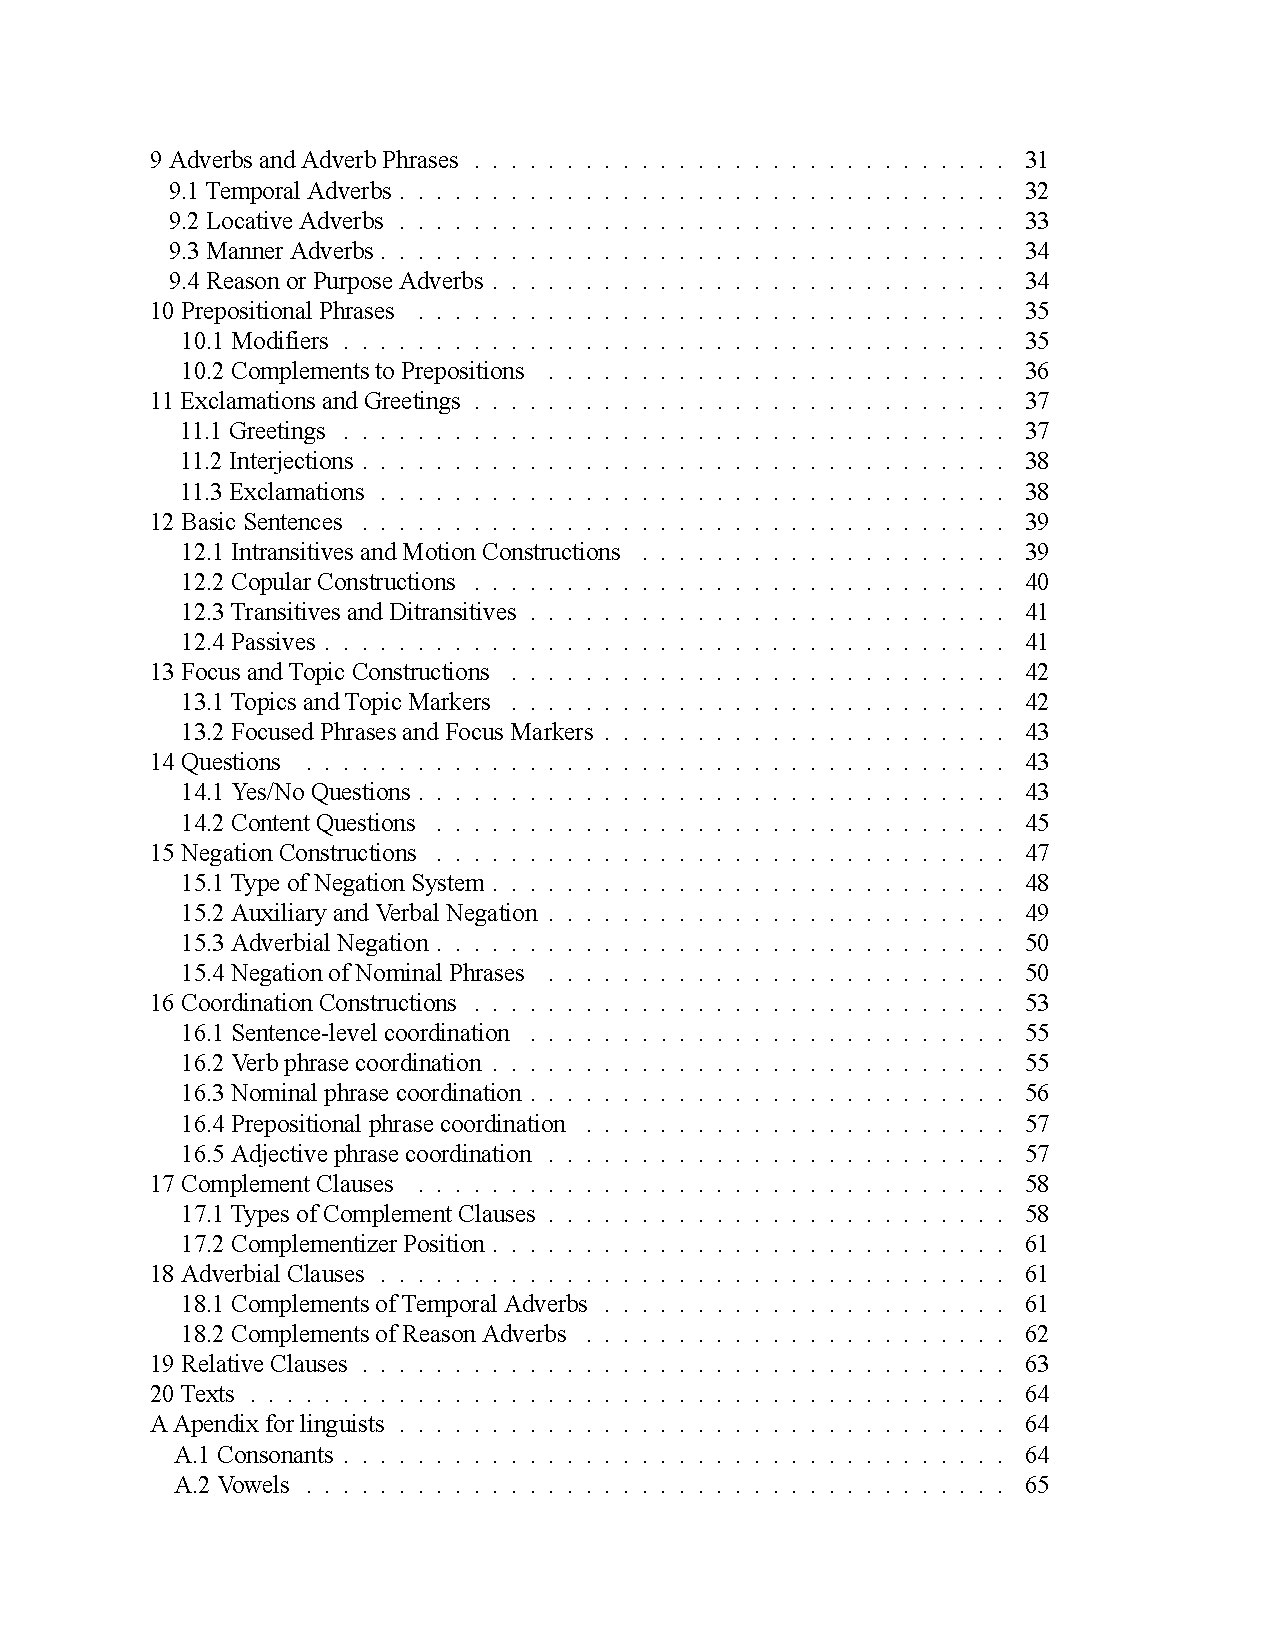
\includegraphics[width=.45\textwidth]{\imgpath/Contents2a.pdf}
\caption{Table of contents for the initial output of one grammar}
\label{xContents}%11
\end{sidewaysfigure}


\subsubsection{Use of XLingPaper}\label{sXLingPaper}
The practical grammar is output in XLingPaper format, which can then be edited as described in sections \ref{sXLingPaperOutputs}-\ref{sXMLMind}.  Before discussing this, we give a brief sketch of the advantages of XLingPaper.

Linguistic documents are by nature complex and also have many conventions. Using WYSIWYG editors like Microsoft Word and Open Officer Writer ``work'' but are not very convenient. As \citet{rSimonsAndBlackSFLF} point out, WYSIWYG editors are ``second wave'' technology. XLingPaper, on the other hand, uses ``third wave'' technology and is designed specifically for linguistic documents.

Linguists commonly face three obstacles in formatting papers. First, all examples are numbered in a paper. If during the writing process the author discovers a need to insert an example, then the numbering of all following examples and all references to those examples within the text need to be re-adjusted. This mechanical change can be both time-consuming and prone to error. Similarly, if the author decides to reorder some examples, then the numbering needs to be adjusted appropriately. XLingPaper provides an automatic way to facilitate such numbering and renumbering. 

Secondly, linguists cite the work of other researchers using a standard citation format. This format functions essentially as an abbreviation or reference to the full citation entry which appears in the references section of the paper. The burden of maintaining consistency between citation and reference typically falls totally on the author. Many a reader has been disappointed to find a citation to a paper in the body of a paper for which there is no entry in the references section. XLingPaper provides an automatic means for a writer to maintain consistency; all citations in the text must have a corresponding entry in the references. Conversely, XLingPaper will include only those entries in the references section which are cited in the text. This latter characteristic implies that one can maintain one master list of references and merely include it in any given paper. Only those references actually cited in the given paper will appear in the references section. 

Thirdly, linguists commonly use a set of abbreviations while glossing examples. They usually include either a list of the abbreviations and their definitions in a footnote, in a special front-matter page, or in a back-matter page. As for citations and references, the burden of maintaining consistency between the abbreviations used in the text and the abbreviations defined in the list typically falls totally on the author. Many a reader has been disappointed to find an abbreviation in a gloss for which there is no corresponding entry in the list of abbreviations. XLingPaper provides an automatic means for a writer to maintain consistency; the author can make it so all abbreviations in the text must have a corresponding entry in the list of abbreviations. Conversely, XLingPaper will include only those abbreviations in the list of abbreviations which are actually used in the text. This latter characteristic implies that one can maintain one master list of abbreviations\footnote{\label{nLeipzig}
   The starter master list which comes with XLingPaper is based on the Leipzig conventions given in  \url{http://www.eva.mpg.de/lingua/resources/glossing-rules.php}.
} 
and merely include it in any given paper. Only those abbreviations actually cited in the given paper will appear in the list of abbreviations. By the way, XLingPaper also creates a hyperlink between the abbreviation in the text and the abbreviation in the list of abbreviations. Thus, a reader can click on the abbreviation and see what it means.

Furthermore, XLingPaper  uses actionable data by marking-up linguistic documents in XML so one can produce multiple outputs from a single input.  As a brief example, the short section shown in Figure \ref{xSVCZSectionsXXE} is how a portion of one XLingPaper document appears in the {\XMLmindXMLEditor}.

\begin{figure}[h]
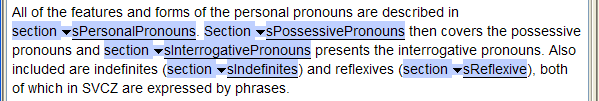
\includegraphics[width=\textwidth]{\imgpath/SVCZSectionsXXE.png}
\caption{A portion of an XLingPaper document in the {\XMLmindXMLEditor}}
  \label{xSVCZSectionsXXE}%12
\end{figure}

When this portion is formatted using the default PDF output format of XLingPaper, it looks like what is given in Figure \ref{xSVCZSectionsDefault}.
  
\begin{figure}[h]
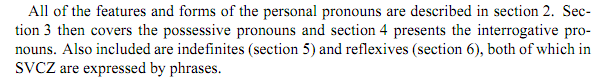
\includegraphics[width=\textwidth]{\imgpath/SVCZSectionsDefault.png}
\caption{Formatted pdf-output of the example in Figure \ref{xSVCZSectionsXXE}}
 \label{xSVCZSectionsDefault}%13
\end{figure}


When this sample document is associated with a publisher style sheet designed for submissions to the {\textit{International Journal of American Linguistics}} (see \citet{rIJALStyleSheet}), this portion will be formatted as in Figure \ref{xSVCZSectionsIJALSubmission}.  Notice that it is double-spaced and that the section numbers are in bold.

\clearpage
\begin{figure}[t]
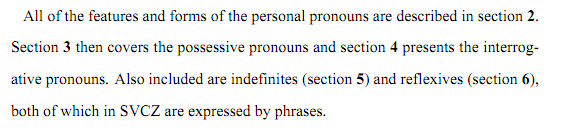
\includegraphics[width=\textwidth]{\imgpath/SVCZSectionsIJALSubmission.png}
\caption{Pdf-output of the example in Figure \ref{xSVCZSectionsXXE} formatted for \textit{IJAL}}
  \label{xSVCZSectionsIJALSubmission}%14
\end{figure}


 


When this sample document is associated with a publisher style sheet designed for the journal {\textit{Language}} (see \citet{rLanguageStyleSheet}), this portion will be formatted as in Figure \ref{xSVCZSectionsLanguage}. Notice that it is single-spaced in a smaller font size, the section numbers are in regular type face, and that rather than using the word ``section,'' it uses the section symbol §.

\begin{figure}[h]
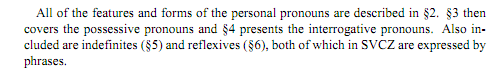
\includegraphics[width=\textwidth]{\imgpath/SVCZSectionsLanguage.png}
\caption{Pdf-output of the example in Figure \ref{xSVCZSectionsXXE} formatted for \textit{Language}}
 \label{xSVCZSectionsLanguage}%15
\end{figure}

 

The three different outputs shown in Figures \ref{xSVCZSectionsDefault}-\ref{xSVCZSectionsLanguage} are all produced without any changes to the main content of the XLingPaper document.  This shows the power of using actionable data.\footnote{\label{nXLingPaperPowerOfActionableData}
   For more on this, see the demonstration movie ``The Power of Actionable Data" on the XLingPaper web site, \url{http://www.xlingpaper.org/?page\_id=14}.
}

XLingPaper works natively on Windows, Mac OS X, and Linux operating systems.\footnote{\label{nXXEOSes}
   This is largely due to the fact that the {\XMLmindXMLEditor} runs natively on these operating systems.
}  
An XLingPaper document can be output in any of five formats:

\begin{itemize}
  \item {Web page (html)}
  \item {PDF (via XeLaTeX; see \url{http://scripts.sil.org/cms/scripts/page.php?site_id=nrsi&id=xetex})}
  \item {PDF (via RenderX; see \url{http://www.renderx.com/})}
  \item {Microsoft Word 2003}
  \item {Open Office Writer}
\end{itemize}

Those who have used XLingPaper have said things like the following quotes:

\begin{itemize}
  \item ``I'm totally hooked on this program now and am generally getting quite comfortable using it.''
  \item It ``has enabled me to be vastly more productive in writing linguistic papers and in dialoguing with linguistic consultants.''
  \item ``I really like using XLingPaper.  It's a much better working space for me than MS Word (partly because I have spent so much time not being productive, in Word, and because of the intimidation of the blank page.)''
  \item ``XLingPaper has been working great, and I've been using it to author \dots{} most of what I write.''
\end{itemize}

To see some sample papers produced via XLingPaper, see Working Papers \# 1, 3, 4, 7, 8, 9, 10, and 13 at \url{http://www.sil.org/mexico/workpapers/WPindex.htm}.

While XLingPaper is a powerful authoring tool for linguistic documents, the user of {PAWS} does not have to learn everything about XLingPaper before s/he can begin editing. This is because {PAWS} already formats the sections, interlinear examples, and tables so that the user only has to key in the glosses or other additional information requested. Further, adding additional description or interlinear examples or tables can be done by simply copying and pasting similar ones already in the document.

\subsubsection{XLingPaper outputs}\label{sXLingPaperOutputs}
As we just mentioned, the output is in XLingPaper format, which allows editing within XML editors, and produces outputs in both HTML (\citet{rW3CHTML} and PDF (\citet{rISOPDF1.4} formats. {PAWS} automatically generates the HTML output for the user's convenience.

The HTML output page corresponding to the input page from Figures \ref{xPossesors1}-\ref{xPossessors3} 
% of section \ref{sPages} 
is shown in Figure \ref{xPossessorsHtml2}.

\begin{figure}
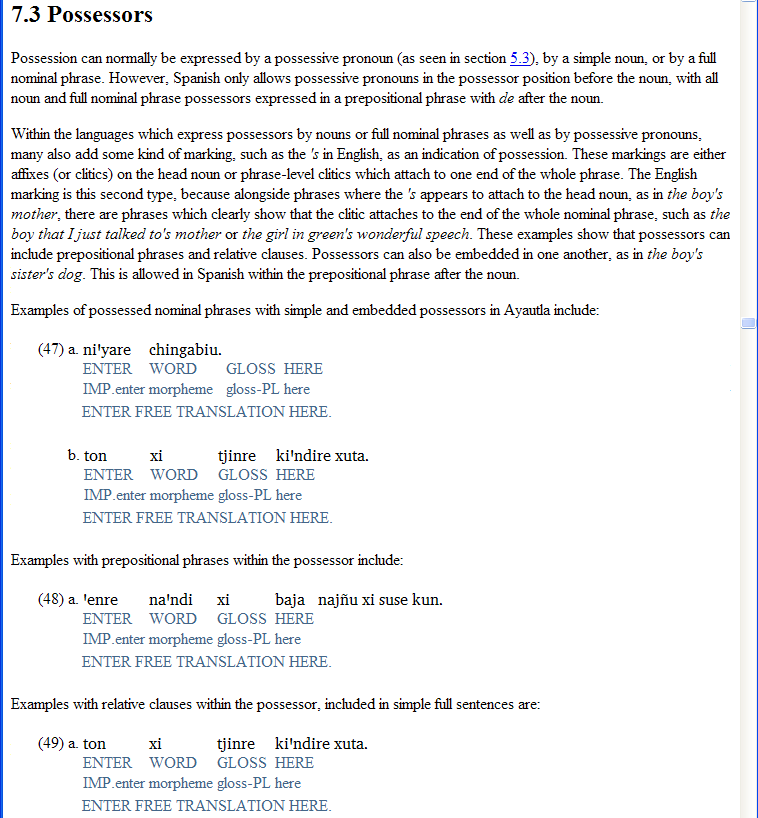
\includegraphics[width=\textwidth]{\imgpath/PossessorsHtml1.png} 
...\\[1em]
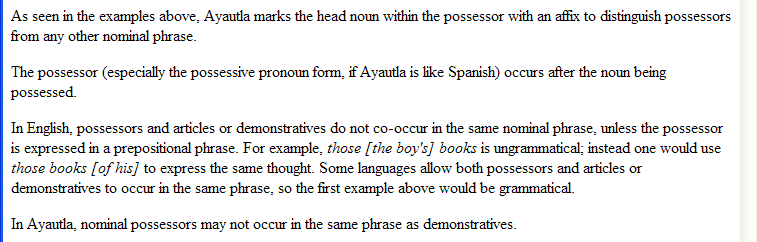
\includegraphics[width=\textwidth]{\imgpath/PossessorsHtml2.png}
\caption{HTML output of the content of Figures  \ref{xPossesors1}-\ref{xPossessors3}}
  \label{xPossessorsHtml2}%17
\end{figure}

While {PAWS} only generates the HTML output, XLingPaper allows for multiple possible PDF outputs.

\subsubsection{{\XMLmindXMLEditor}}\label{sXMLMind}
We have found that using XLingPaper with the {\XMLmindXMLEditor} is the most convenient.\footnote{\label{nXXE}
   See \url{http://www.xmlmind.com/xmleditor/} for more on this exceptional structured editor.
} 
This is because the {\XMLmindXMLEditor} hides the XML from the user. In addition, the XLingPaper configuration files for the {\XMLmindXMLEditor} provide many other capabilities that makes it convenient for the author.

What the user sees within the {\XMLmindXMLEditor} for the first part of the same page we illustrated above in Figures \ref{xPossesors1}-\ref{xPossessors3} is given in Figure \ref{xXXE1}.

\clearpage
\begin{figure}[h]
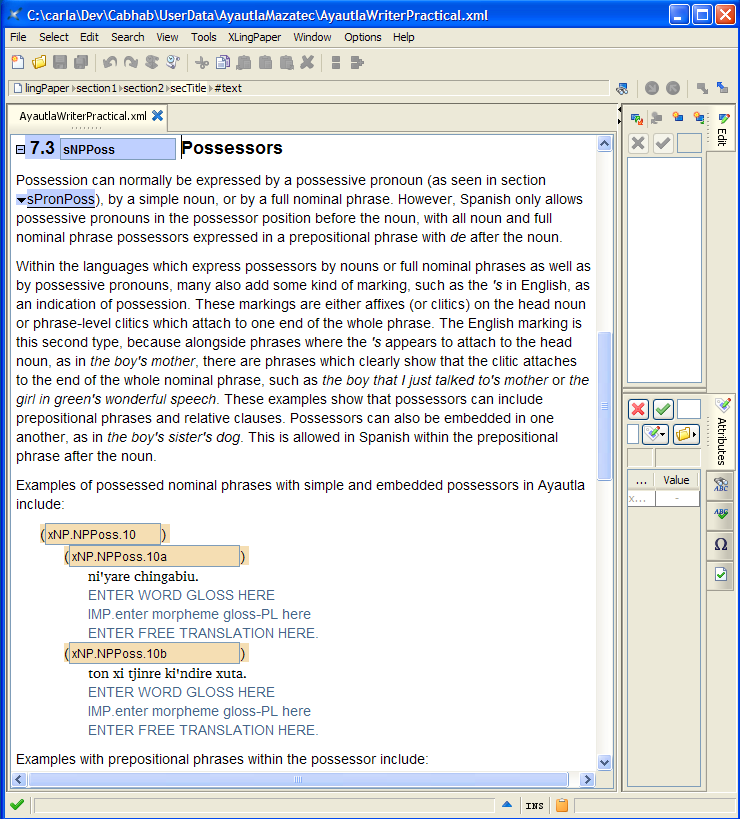
\includegraphics[width=\textwidth]{\imgpath/XXE2.png}
\caption{Screenshot of the {\XMLmindXMLEditor}}
\label{xXXE1}%18
\end{figure}
\clearpage
The section level 2 item begins the portion, followed by several paragraphs of descriptive prose. It ends with two sets of interlinear examples. These have the four lines discussed in section \ref{sPracticalStructure}. The editor allows the user to type in the information asked for in blue, as well as to add additional data and/or prose as appropriate.

\section{How it works}\label{sComp}
Having described what {PAWS} entails, we turn now to describing how it works. 


\subsection{The configuration files}\label{sConfig}
The {PAWS} program consists of a shell or host program (called \textsc{cabhab}) which has an embedded web browser and also processes a set of configuration files. These files determine the user interface such as menu items, define sets of transforms to apply to the answer file, and also determine what shows in the embedded web browser.

There are several sets of configuration files. 

\subsubsection{Controlling the shell}\label{sConfigCabhab}
There is a configuration file that controls what the {cabhab} shell shows the user and also how the answer file is transformed into various outputs.

For example, the menu items are defined as shown in \xref{xConfigMenuItems}.

\ea  \label{xConfigMenuItems}%19
\begin{verbatim}
<menubar>
   <menu id="File" label="File">
      <item command="CmdNewLanguage" defaultVisible="true"/>
      <item command="CmdOpenLanguage"/>
      <item command="CmdCloseLanguage"/>
      <item command="CmdSaveLanguageAs"/>
      <item label="-"/>
      <item command="CmdGenerateFiles"/>
      <item label="-"/>
      <item command="CmdLanguageFileLocations"/>
      <item label="-"/>
      <item command="CmdExit"/>
   </menu>
   <menu id="Edit" label="Edit">
      <item command="CmdCut"/>
      <item command="CmdCopy"/>
      <item command="CmdPaste"/>
      <include path="Extensions/*/MainConfigurationExtension.xml" 
        query="root/menuAddOn/menu[@id='Edit']/*"/>
   </menu>
   <menu id="Language" label="Language">
      <item command="CmdLanguageProperties"/>
      <item command="CmdLanguageFileLocations"/>
      <include path="Extensions/*/MainConfigurationExtension.xml" 
        query="root/menuAddOn/menu[@id='Edit']/*"/>
   </menu>
   <menu id="View" label="View">
      <item label="Show Toolbar" boolProperty="ShowToolbar" 
            command="CmdShowToolbar"/>
      <item label="Show Status Bar" boolProperty="ShowStatusBar"
            command="CmdShowStatusBar"/>
      <item label="-"/>
      <item command="CmdBack"/>
      <item command="CmdForward"/>
      <item command="CmdRefresh"/>
   </menu>
   <menu id="Help" label="Help">
      <item id="Resources" command="CmdResources"/>
      <item label="-"/>
      <item id="About" command="CmdAbout"/>
   </menu>
</menubar>
\end{verbatim}
\z

 The commands referred to by <item> elements are defined in the configuration file as given in example \xref{xConfigCommands}.

\ea  \label{xConfigCommands}%20
\begin{verbatim} 
<commands>
   <command id="CmdNewLanguage" label="Create _New 
            Language" shortcut="Ctrl+N" 
            message="NewLanguage" icon="New"/>
   <command id="CmdOpenLanguage" label="Open Language" 
            message="OpenLanguage" shortcut="Ctrl+O" 
            icon="Open"/>
   <command id="CmdCloseLanguage" label="Close Language" 
            message="CloseLanguage"/>
   <command id="CmdGenerateFiles" label="Generate Files"
            message="GenerateFiles" shortcut="Ctrl+S" 
            icon="Save"/>
   <command id="CmdSaveLanguageAs" label="Save Language 
            As" message="SaveLanguageAs"/>
   <command id="CmdExit" label="E_xit" 
            message="ExitApplication"/>
   <command id="CmdCopy" label="Copy" message="EditCopy" 
            icon="Copy" shortcut="Ctrl+C"/>
   <command id="CmdCut" label="Cu_t" message="EditCut" 
            icon="Cut" shortcut="Ctrl+X"/>
   <command id="CmdPaste" label="Paste" message="EditPaste" 
            icon="Paste" shortcut="Ctrl+V"/>
   <command id="CmdLanguageProperties" label="Properties" 
            message="LanguageProperties"/>
   <command id="CmdLanguageFileLocations" label="File _Locations" 
            message="LanguageFileLocations"/>
   <command id="CmdBack" label="Back" message="BrowserBack" 
            icon="Back" shortcut="Alt+Left"/>
   <command id="CmdForward" label="Forward" message="BrowserForward" 
            icon="Forward" shortcut="Alt+Right"/>
   <command id="CmdRefresh" label="Refresh" message="BrowserRefresh" 
            icon="Refresh" shortcut="F5"/>
   <command id="CmdAbout" label="About PAWS" message="AboutPage"/>
   <command id="CmdResources" label="Resources" 
            message="ResourcesPage"/>
   <command id="CmdShowToolbar" label="Show Toolbar" 
            message="ShowToolbar"/>
   <command id="CmdShowStatusBar" label="Show Status Bar" 
            message="ShowStatusBar"/>
</commands>
\end{verbatim}
\z


 The message attribute refers to code in the {cabhab} program which is run when that command is invoked.

 The set of transforms which are used to produce the various outputs are defined as illustrated in example \xref{xConfigAnswerFileTransforms}. Only the one for the practical grammar output (in English) is shown. The others are similar.

\ea  \label{xConfigAnswerFileTransforms}%21
\begin{verbatim}
 
<answerFileTransformSets>
   ...
   <answerFileTransformSet>
      <transform 
        file="Transforms/PAWSSKMasterWriterPracticalMapper.xsl"
        resultFileFromAnswerFile="//language/writerPracticalFile" 
        ext="xml" saveResult="true"
        applyTransformWhenXPath=
            "/paws/\@outputWriterPractical[.='True']"
        insertConfigPathInTransformDOCTYPE="true" 
        replaceDOCTYPE="&lt;!DOCTYPE 
        lingPaper PUBLIC &quot;-//XMLmind//DTD XLingPap//EN&quot; 
        &quot;XLingPap.dtd&quot;&gt;" lang="en">
         <xsltParameters>
            <param name="prmSDateTime" value="fake"/>
            <param name="prmSVersionNumber" value="fake"/>
         </xsltParameters>
      </transform>
      <transform file="Transforms/XLingPap1.xsl" 
        resultFileFromAnswerFile="//language/writerPracticalFile" 
        ext="htm"
        applyTransformWhenXPath=
            "/paws/@outputWriterPractical[.='True']"/>
   </answerFileTransformSet>
   ...
</answerFileTransformSets>
\end{verbatim}
\z

\subsubsection{Web page description}\label{sConfigWebPage}
The second set of configuration files are the web page descriptions. The development of each web page used in PAWS was done by a non-programmer linguist, who wrote XML files describing the content of the page. Example \xref{xSamplePageDescription} shows a portion of the XML description used to produce the page shown in Figures \ref{xPossesors1}-\ref{xPossessors3}.

\ea  \label{xSamplePageDescription}%22
\begin{verbatim}
<page id="NPPossessors" count="1/2">
   <title level="2">Nominal Phrases - Possessors</title>
   <introduction> 
      The next type of modifier to consider is 
      possessors. Possession can normally be expressed by a
      possessive pronoun (to be addressed in <section 
      number="7">Pronouns</section>) or by a simple noun... 
      a prepositional phrase with <example>de</example> 
      after the noun.<br/>... These examples show that 
      possessors can include pre/post-positional phrases 
      and relative clauses. 
    </introduction>
   <form section="np">
      <prompt>
        Think about how possession is expressed in your
        language. ...
      </prompt>
      <prompt> 
        Key some examples with simple and embedded 
        possessors here:
      </prompt>
      <textBox id="NPPossEmbeddedExample"
               dataItem="embeddedExample"/> 
       <radioGroup>
         <groupName dataItem="possMarked" default="no">
          RNPPossMarked
         </groupName>
         <prompt>
            Based on your examples, does your language have 
            any special marking to distinguish possessors 
            from any other nominal phrase?
         </prompt>
         <radio id="NPPossMarkedNo" dataValue="no">
            No, there is no special marking
         </radio>
         <radio id="NPPossMarkedYesAffix" dataValue="yesAffix">
            Yes, the head noun within the possessor is 
            syntactically marked via an affix
         </radio>
         <radio id="NPPossMarkedYesClitic" dataValue="yesClitic">
            Yes, the whole possessive phrase is syntactically 
            marked via a phrasal clitic
          </radio>
         ...
      </radioGroup>
   </form>
</page>

\end{verbatim}
\z

An XSLT transform then produces the web page itself on the fly while the user is running {PAWS}.

\subsubsection{Writer output description} \label{sConfigWriterOutput}
  
The next set of configuration files describes a given writer output.

The writer output was developed similarly: the linguist described the desired output in XML and then this XML was transformed into the XSLT that {PAWS} uses. For example, the portion of XML shown in \xref{xPossessorPracticalWriter} shows part of what ends up producing the kind of output given in Figure \ref{xPossessorsHtml2}.\footnote{\label{nContentElement}
   The use of the <content> element instead of plain PCDATA is a result of how the XSLT to transform this XML to XSLT was written: if one used PCDATA, the resulting XSLT would be incorrect.
}

\ea  \label{xPossessorPracticalWriter}%23
\begin{verbatim}
<section2 id="sNPPoss"> 
   <secTitle>Possessors</secTitle> 
   <p> 
      <content>
          Possession can normally be expressed by a 
          possessive pronoun (as seen in section 
      </content> 
      <sectionRef sec="sPronPoss"/> 
      <content>
          ), by a simple noun, or by a full nominal 
          phrase. However, Spanish only allows 
          possessive pronouns in the possessor 
          position before the noun, with all noun 
          and full nominal phrase possessors expressed 
          in a prepositional phrase with 
      </content>
      <langData>de</langData> 
      <content> after the noun.</content> 
   </p>
   ... 
   <p> 
      <content>
          Examples of possessed nominal phrases with 
          simple and embedded possessors in 
      </content>
      <langName/>
      <content> include:</content>
   </p> 
   <example>
      <interlinear exampleLoc="np/embeddedExample"/>
   </example> 
   ... 
   <p> 
   <content>As seen in the examples above, </content>
      <langName/>
   <content/> 
   <case element="np" attr="possMarked"> 
      <caseText value="no"> 
          does not have any special marking to 
          distinguish possessors from any other nominal 
          phrase.
      </caseText> 
      <caseText value="yesAffix"> 
          marks the head noun within the possessor with 
          an affix to distinguish possessors from any 
          other nominal phrase.
      </caseText> 
      <caseText value="yesClitic"> 
          marks the whole possessive phrase with a phrasal 
          clitic to distinguish possessors from any other 
          nominal phrase.
      </caseText>
   </case>
   <content/> 
\end{verbatim}
\z

\subsection{Process for producing writer output}\label{sProcessProducingWriterOutput}
The overall process for producing the writer output is illustrated in Figure \ref{xWriterToOutput}.

\begin{figure}
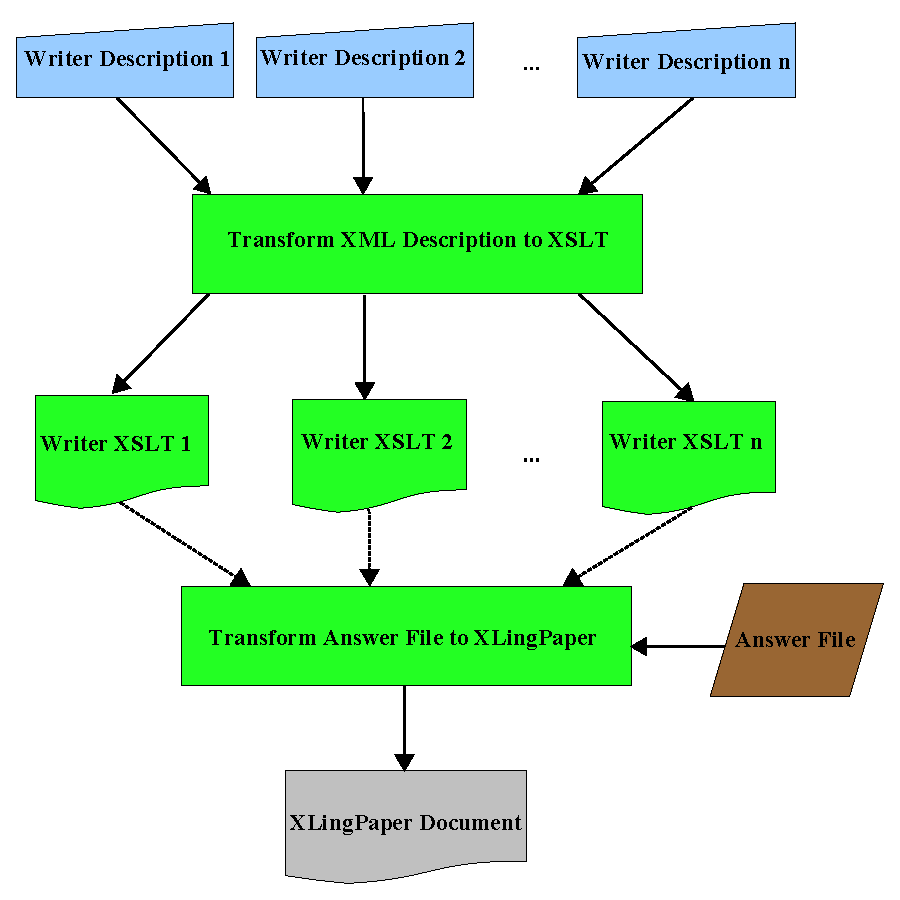
\includegraphics[width=\textwidth]{\imgpath/WriterXMLtoXSLFlow3NewText.pdf}
\caption{Process of producing XLingPaper} 
 \label{xWriterToOutput}%24
\end{figure}

The linguist writes several writer description XML files, each of which must conform to a Document Type Definition \citep[also known as a DTD; see ][]{rW3CDTD}. Each such file typically describes a section or a sub-section of the intended output. Each of these writer description files is then passed through an XSLT transform to produce the corresponding writer XSL file.\footnote{\label{nWriterToXSLDoneOnce} 
 This is done only once during the development process. The individual writer XSL files are then included in the installation package as part of {PAWS}.
} 
These are combined together in the master XSLT writer transform. The PAWS program then applies the answer file to this combined transform to produce the XLingPaper document output.

\subsection{Choice of outputs} \label{sOutputs}
As noted above in section \ref{sPages}, through the use of actionable data, a single set of answers to questions and example data that the user enters can provide either a PC-PATR grammar file and test data for syntactic parsing or a choice of two styles of a grammar write-up.

This grammar write-up is an XML file in XLingPaper format, so it is ready for electronic publishing.\footnote{\label{nMukurtu}
 One reviewer of an earlier version of this paper mentioned the Mukurtu repository system (see \url{http://www.mukurtu.org/}). One could easily put the output of the edited XLingPaper result of {PAWS} on such a site. Another reviewer noted that a wiki rather than XML would be a possible target for a language community. We acknowledge this possibility with thanks. Since XLingPaper data is actionable, it is at least conceivable that one could create an XSLT transform that would convert the XLingPaper XML document to wiki pages. One could then post these pages to a wiki site, enabling the language community to refine the result.
} 
See examples in section \ref{sXLingPaper} above.

\subsection{Localization}\label{sLocal} 
The original grammar write-up included in PAWS closely follows the order and style of the user interface pages within PAWS, so it is a descriptive, pedagogical grammar comparative to English. This has been customized with the addition of the option of producing a practical grammar style write-up. Currently, the practical grammar is available in English and in Spanish. The process of translating the practical grammar output involves making a new copy of the XML writer description files, such as the one shown in \xref{xPossessorPracticalWriter}, and translating the text.

SIL International uses such practical grammars in Mexico, written in Spanish. (See \citet{rHollenbach} as well as \citet{rPickettBlackMarcial} and \citet{rPersonsBlack} for examples.) Therefore, the practical grammar option has been translated into Spanish and the translation of the user interface is in process, to allow greater use throughout the Spanish-speaking world. Similar localization for other languages could be done in the future.

Additional customization is possible by the user (with configuration files to generate a transform), since PAWS employs XML technologies.

\section{Conclusion}\label{sConc}
This paper has shown how using XML technologies to produce an expert system allows PAWS to meet multiple needs and produce multiple outputs. While originally developed for syntactic parsing, it can also be used to produce practical grammars, with the more complex instructions hidden from the user. This practical grammar option, especially coupled with localization into the national language, allows linguistically-aware native speakers of indigenous languages to partner with linguists in the task of documenting and describing the minority languages of the world and providing useful grammars for each language community.

Workshops on grammar writing are much more productive by beginning with PAWS. In such workshops, the participants all complete PAWS and then are taught how to edit the output using XLingPaper. From then on, the workshop can move to dealing with any language-specific phenomena not covered in PAWS. The participants can be taught how to search for the needed data, how to analyze it and then how to write it up in the grammar.

Though the grammar drafts output by PAWS have a template-like quality, they are simply a big head start on writing the grammar. After editing and enhancing the grammar using XLingPaper, a unique description of the particular language can be produced.

\setcounter{secnumdepth}{3}
